% file: graph-decomposition/hamiltonian-path-dag.tex

\documentclass[tikz]{standalone}
\usetikzlibrary{positioning, arrows.meta, chains}

\begin{document}
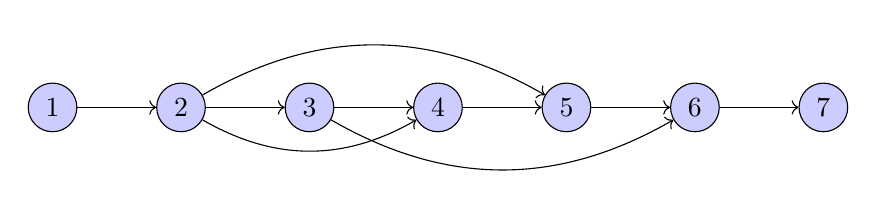
\begin{tikzpicture}[node distance = 1.00cm, 
      every node/.style = {draw, circle, fill = blue!20},
      every join/.style = {->},
      every edge/.style = {draw, ->},
      start chain = path]

      \foreach \i in {1, ..., 7} {
	\node [on chain, join] {\i};
      }

      \path (path-2) edge[bend left = 30] (path-5)
	    (path-2) edge[bend right] (path-4)
	    (path-3) edge[bend right = 30] (path-6);
\end{tikzpicture}
\end{document}
